% Set the document's formatting to "report"
\documentclass[openright]{report}

% Include titlesec[personalized chapters], graphicx[images], tocbibind[bibliography in toc], comment[comment paragraphs], lmodern/fontend[fix tilde typesetting], afterpage[insert blankpages], etoolbox[flawless page numbering], blindtext[lorem ipsum], mathtools[math symbols], listings/alloy/color[alloy syntax], fp[variables evaluation] and glossaries/imakeidx[glossary] packages
\usepackage[utf8]{inputenc}
\usepackage{titlesec}
\usepackage{graphicx}
\usepackage{tocbibind}
\usepackage{comment}
\usepackage{lmodern}
\usepackage[T1]{fontenc}
\usepackage{afterpage}
\usepackage{etoolbox}
\usepackage{blindtext}
\usepackage{mathtools}
\usepackage{listings}
\usepackage{color}
\usepackage[nomessages]{fp}
\usepackage[nonumberlist,acronym,toc,xindy]{glossaries}
\makeglossaries
\usepackage[xindy]{imakeidx}
\makeindex


\definecolor{alloy-keyword}{rgb}{0.23, 0.23, 0.7}
\definecolor{alloy-comment}{rgb}{0.18, 0.64, 0.18}
\definecolor{alloy-string}{rgb}{0.71, 0.18, 0.71}

% Patch page numbering
\patchcmd{\abstract}{\titlepage}{\thispagestyle{empty}}{}{}
\patchcmd{\endabstract}{\endtitlepage}{\clearpage}{}{}

% Create new \blankpage command
\newcommand\blankpage{%
    \null
    \thispagestyle{empty}%
    \addtocounter{page}{-1}%
    \newpage}

% Edit title styling
\titleformat{\chapter}{\Huge\bfseries}{}{0pt}{\Huge}

% Set images path
\graphicspath{{../resources/images/}}

% Create auxiliary variables for worktime and version tracking 
\def \worktimeNicola {20}
\def \worktimeGiacomo {20}
\FPupn{worktimeTotal}{worktimeNicola worktimeGiacomo + 0 round}
\FPupn{version}{1.0}


\begin{document}

	\begin{titlepage}
		\centering

\includegraphics[width=0.50\textwidth]{polimi}\\\vspace{0.25cm}
{\scshape\LARGE Politecnico di Milano\par}\vspace{0.25cm}
{\scshape\Large Software Engineering II project: PowerEnjoy\par}\vspace{1.5cm}
{\huge\bfseries Code Inspection \par}\vspace{1cm}
{\large Gregori Giacomo and Ruaro Nicola\par}\vfill

% Bottom of the page
{\large \today \\Version \version}

	\end{titlepage}

	% Change page numbering to uppercase roman for introductory pages
    \pagenumbering{Roman}

    \tableofcontents

    \newpage
    \blankpage
    \begin{abstract}
		This document provides a detailed description of the Integration Test's planning for the PowerEnJoy system. It is based on the RASD and DD documents presented in the previous deliveries and must explain to the developement team how to test the system.

	\end{abstract}

	% Change page numbering to arabic for the rest of the document
	\pagenumbering{arabic}

    \chapter{Introduction}
    	\section{Scope of the System}
PowerEnJoy is a car-sharing service based on mobile and web applications which should allow users to reserve vehicles and use them.
\\TODO: brief architecture/algorithms/UI description
\section{Document Structure}
\begin{description} 
	\item[Introduction: ] In this chapter an introduction to the system and the Design Document is given.
	\item[Architectural Design: ] In this section an overall description of the architecture is given, it is structured into N different parts: 
		\begin{itemize}
			\item Overview: High-level components and their interaction
			\item Component view
			\item Deployment view
			\item Runtime view
			\item Component Interfaces
			\item Selected architectural styles and patterns
			\item Other design decisions
		\end{itemize}
	\item[Algorithm Design: ] In this chapter the implemented algorithms are discussed and presented using flow-charts and pseudo-code in order to ease the comprehension and focus on the functionality.
	\item[User Interface Design: ] In this section the main choices in User Interface and User Experience design are discussed.
	\item[Requirements Traceability: ] In this section a clear link between requirements specification (RASD) and design decisions (DD) is created.
\end{description}

	\chapter{Architectural Design}
		\section{Overview: High-level components and their interaction}
A brief description of the general design context, the general approach and the overall design of the system with its processes is presented in this section of the DD.
\\Our system will be developed as a 4-tierrd JEE application, divided as Client Tier, Web Tier, Business Tier and the EIS Tier. %3-Tier???
\\The application is distributed over three locations: client machines, the Java EE server machine, and the database.
\\The mobile and web applications in particular are thin since data operations will be computed by a central server; in this way there is no heavy load on user side clients. We think that this is the most feasible approach because the two applications have the same goals. 


The diagram below provides a better understanding of the components of our system, highlighting the interactions in the architecture.
%\subsubsection{Architecture Component Diagram}
\begin{figure}[!h]
  \centering
  \vspace{0.2cm}
  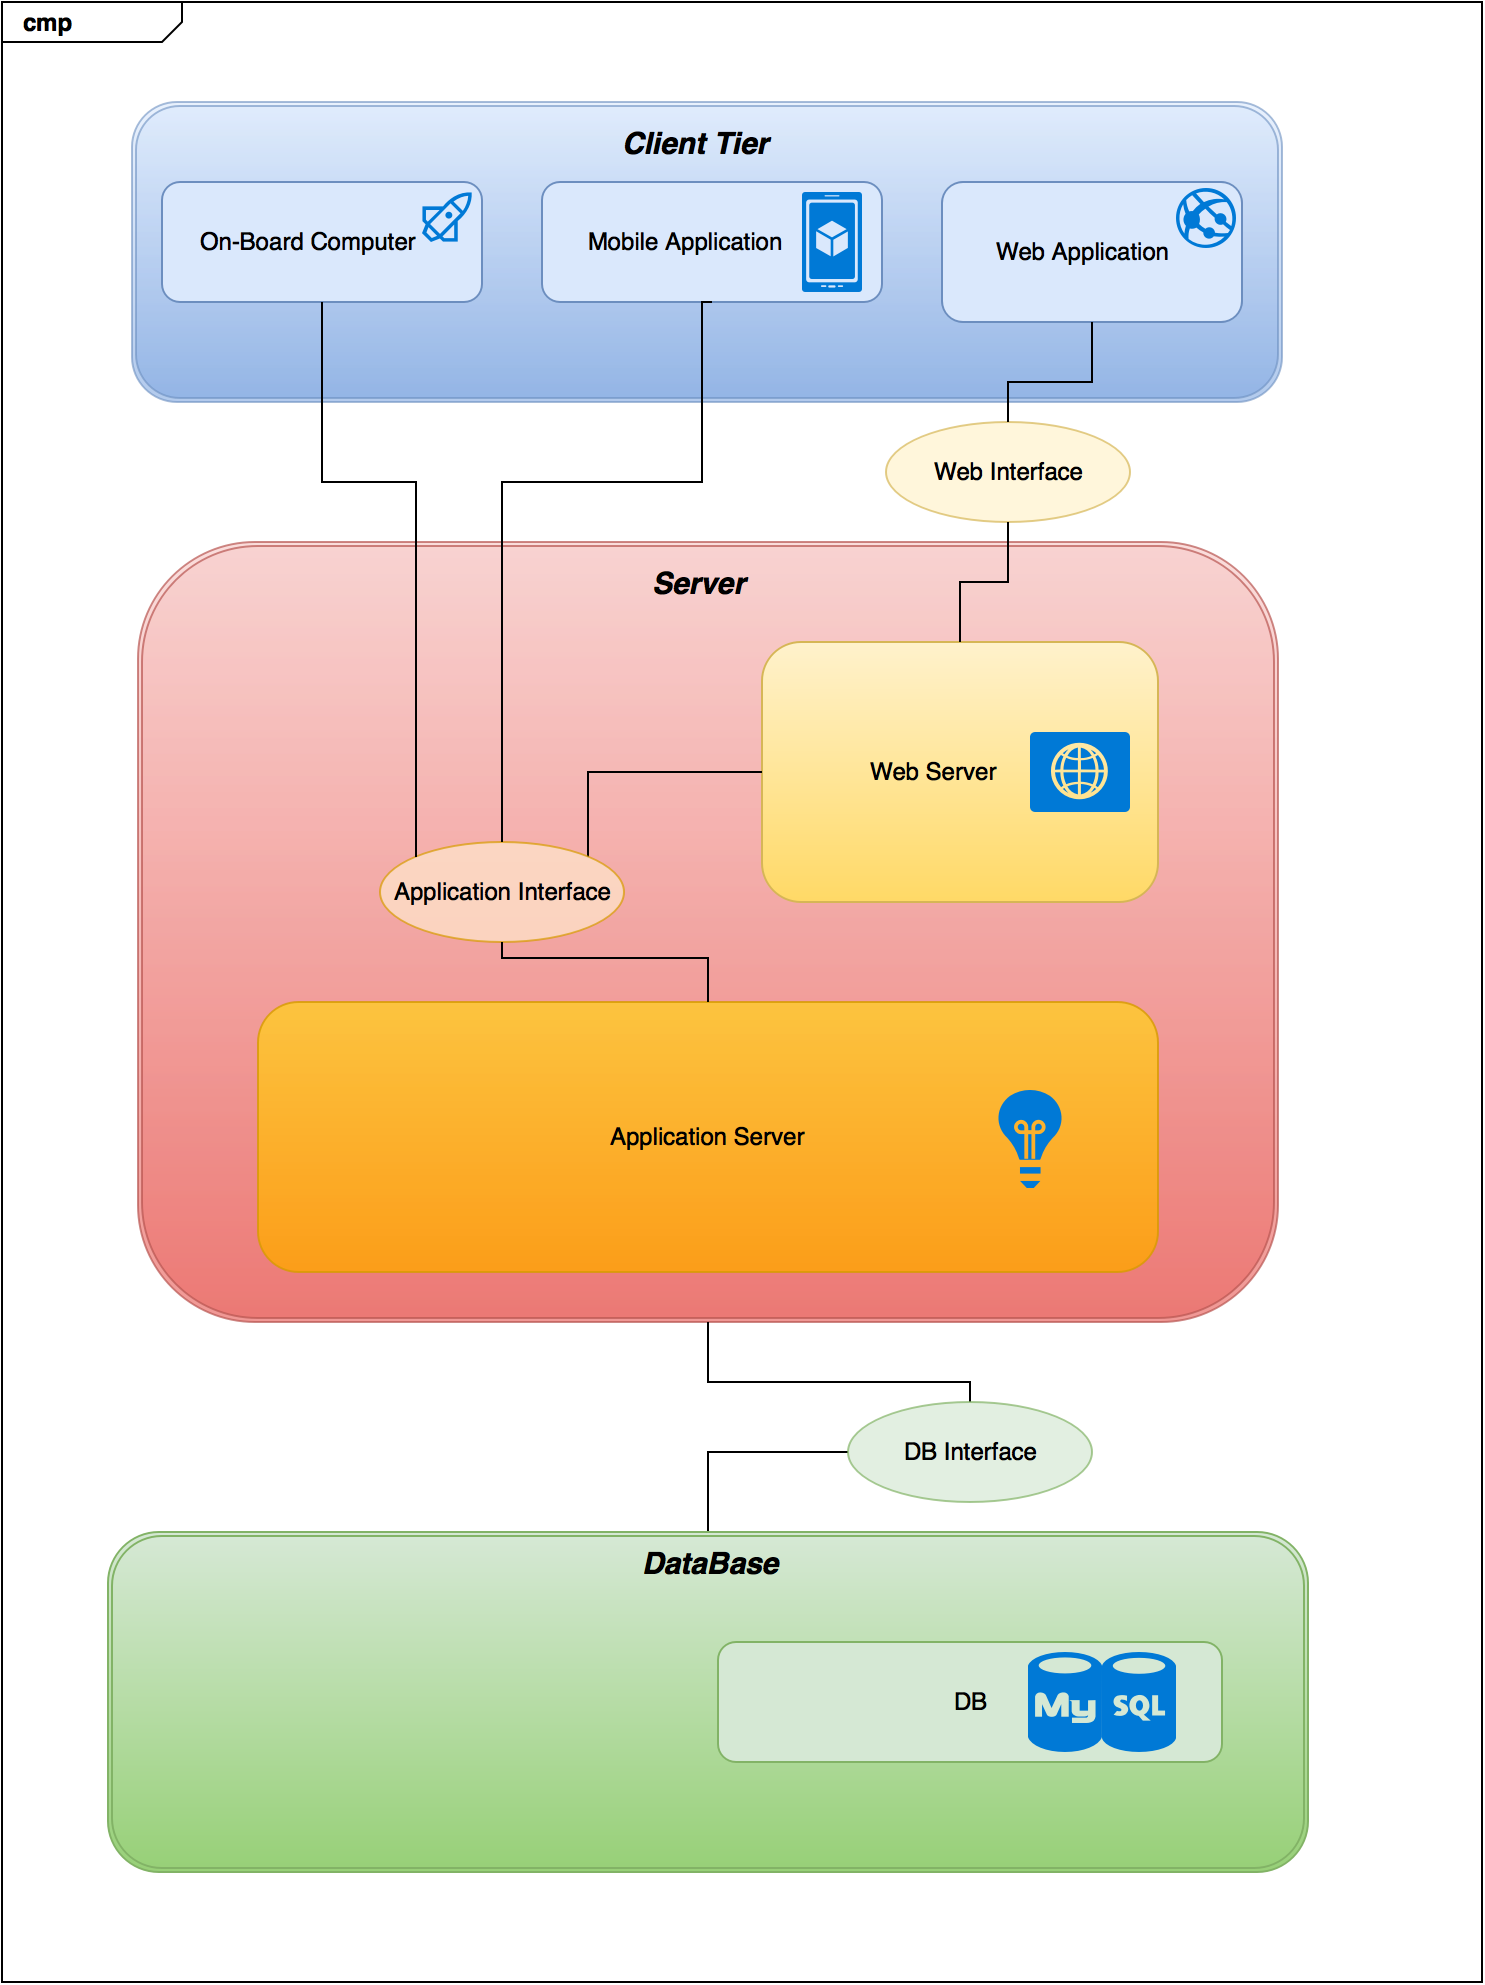
\includegraphics[width=0.6\textwidth]{/DD/4-Tier_Architecture}\\%TODO: add java beans and check the number of tiers
  \vspace{0.4cm}
  %\caption{Mockup for the login mobile page} 
  \label{fig:4-Tier_Architecture} 
\end{figure}

This represent a high level view of the design of the system, were is highlighted the distribution of the system over the three locations and the interaction between the different tiers thanks to their interfaces.
\\The Client Tier is composed by the On-board computer, the mobile application and the web application.
\\The Web Tier and the Business Tier are inside the server machine. We can observe that the Web application need to interact with the Web Server before to access to the Application server while the mobile application has a direct access to it.
\\The EIS Tier consists in a database that store all the system's data and interact through the DB Interface with the server.

\section{Component view}
\subsection{System components}
To define and easily understand what kind of functionalities must be implemented in our system we decided to decompose PowerEnJoy logically into components. Then it is analysed each component and the interaction that it has with the other components, so the common parts can be identified if present. The components are studied to be reusable and easily adaptable in other applications.
%We have decided to decompose PowerEnJoy in different components in order to make it easy to understand what kind of functionalities must be implemented and to separate them, logically, in groups, to state clearer their interaction. The analysis of each component will give us the possibility to find common parts, if there are, and reuse them. 
\\The identified components are:
\begin{itemize}
	\item Access functionalities: provide sign-up to guests and log-in to users. They also allow credentials retrieving.
	\item Profile functionalities: provide the possibility for an user to modify her personal information.
	\item Reservation of the car: this functionality allows users to localize and reserve an available car.
	\item Ride functionalities: provide the possibility to unlock and lock of the car. Then all the system functions related with the ride are allocated here. %to change???
	\item Notification functionalities: provide the visualization of users' notifications, related to payments and reservations.%something else?
	\item Payments functionalities: provide the application of discounts or fees to a ride and menage the process related with the payments.
\end{itemize}

\subsection{Database components}
In particular the data stored in the database will be split through different subcomponents that identified the main entities of our system:
\begin{itemize}
	\item User  %location is not necessary, if a reservation is active we need a tag to indicate it
	\item Vehicle 
	\item SafaArea\&ChargingStation
	\item Reservation 
	\item Ride
	\item Payment  
	\item Notification 
\end{itemize} %something else??

The designed model for persistent data is provided here in a ER diagram in order to better analyze the motivations of our design. That's the representation of the database model:
\begin{figure}[!h]
  \centering
  \vspace{0.2cm}
  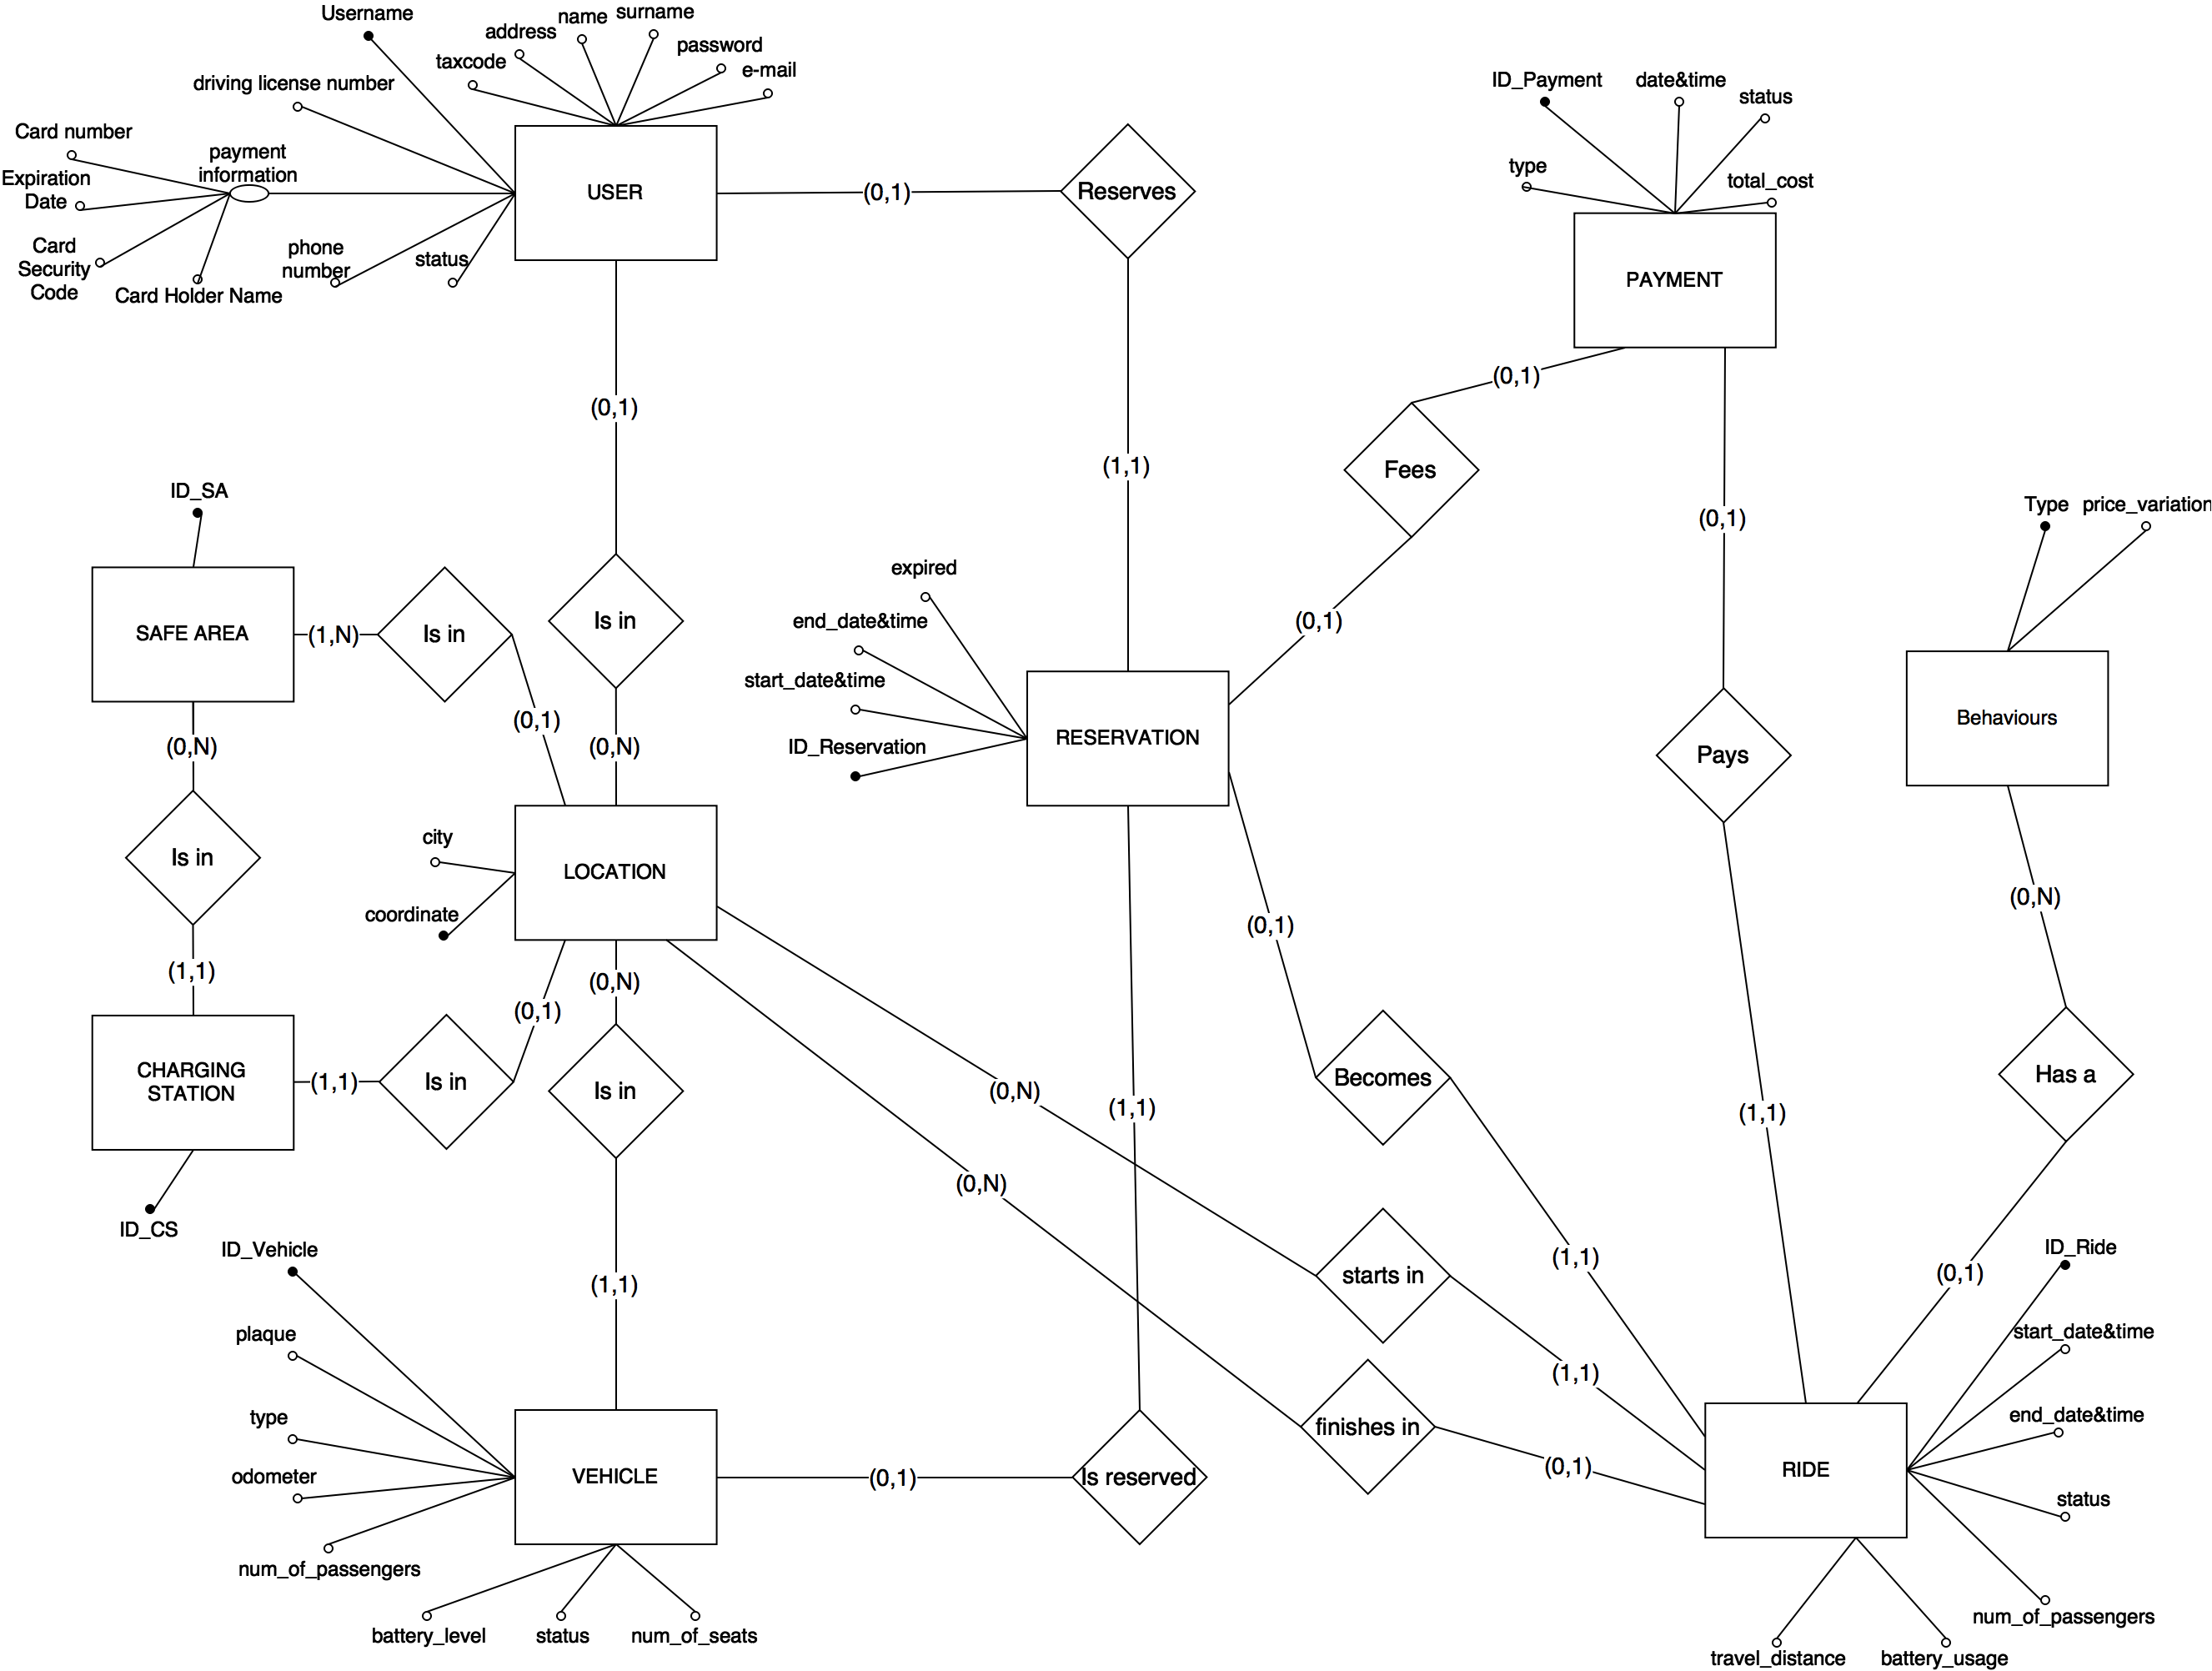
\includegraphics[width=0.7\textwidth]{/DD/ER_Diagram}\\%TODO: add java beans and check the number of tiers
  \vspace{0.4cm}
  %\caption{Mockup for the login mobile page} 
  \label{fig:ER_Diagram} 
\end{figure}

 And this is the relation schema associated with the ER diagram.
\begin{itemize} %TO CHECK WITH THE ER
	\item{User (\underline{ID\_User}, e-mail, pwd, driving\_license, name, surname, payment\_information, location, status)} %status: reserving, riding, free
	\item{Vehicle (\underline{ID\_Vehicle}, plaque, type, odometer, battery\_level, location, status, num\_of\_seats, num\_of\_passengers) }
	\item{SafaArea\&ChargingStation (\underline{location, type}, num\_of\_cars, city)} %type A=Safe Area, B=Charging Station, C=both
	\item{Reservation (\underline{ID\_reservation}, \textit{ID\_User}, \textit{ID\_Vehicle}, start\_date\&time, status)}
	\item{Ride (\underline{ID\_Ride}, \textit{ID\_User}, \textit{ID\_Vehicle}, \textit{ID\_Reservation}, \textit{ID\_Payment}, start\_date\&time, end\_date\&time, status, num\_of\_passengers, travel\_distance, star\_location, end\_location, battery\_usage )}
	\item{Payment (\underline{ID\_Payment}, \textit{ID\_User}, date\&time, total\_cost, fee\_or\_discount, final\_cost, status)}
	\item{Notification (\underline{ID\_Notification}, \textit{ID\_User}, type, date\&time, content)}
\end{itemize}

%TODO: write a little description of each entity, describing the attributes and the possible combinations

\section{Deployment view}
The hardware topology is described here, highlighting components and their relationships. The software parts are deployed in or-
der to have the system working.
\\As previously see in the Overview the system will run thanks of 4 main components:
\begin{itemize}
	\item{The client device, where an User can interact with the system. There are different GUI that renders the web or mobile pages of our system, differentiating between On-board computer, mobile application and web application.}
	\item{ The Web Server is needed for those who are connected to the system with a computer. It establishes a secure internet connection through the HTTPS protocol.}
	\item{The Application Server is the core of our system. Here we have the Business Logic, where the whole system computation is
made.}
	\item{In the Database all the information of the system are stored. It's accessible only by the Application Server that store and take data from there.}
\end{itemize} 

%TO DO schema Deployment View

\section{Runtime view}
In order to state the interaction between the different components of the system here are presented some sequence diagrams.
\\The sequence diagrams highlight the part of the system that interact for implement a function and the messages exchanged between them.
\\In this document are analyzed - different sequence diagrams: %decide the number
\begin{itemize}%TODO
	\item %TODO
\end{itemize} 



\section{Component Interfaces}
	\blindtext
\section{Selected architectural styles and patterns}
	\blindtext
\section{Other design decisions}
	\blindtext

    \chapter{Algorithm design}
    	\blindtext

    \chapter{User interface design}
    	\section{Mockups}
	Mockups for the mobile and web application have been presented and discussed in the RASD. 
	\\TODO: maybe some mockups for the on-board computer should be presented here

\section{UX Diagrams}
	In this section User eXperience diagrams are presented with the intent of defining UI's screens and their interactions.
	\\As stated in the RASD web and mobile application are almost identical and will be treated as a unique application from the UX point-of-view.

	\subsection{On-Board application}
		\begin{figure}[!ht]
		  \centering
		  \vspace{0.2cm}
		  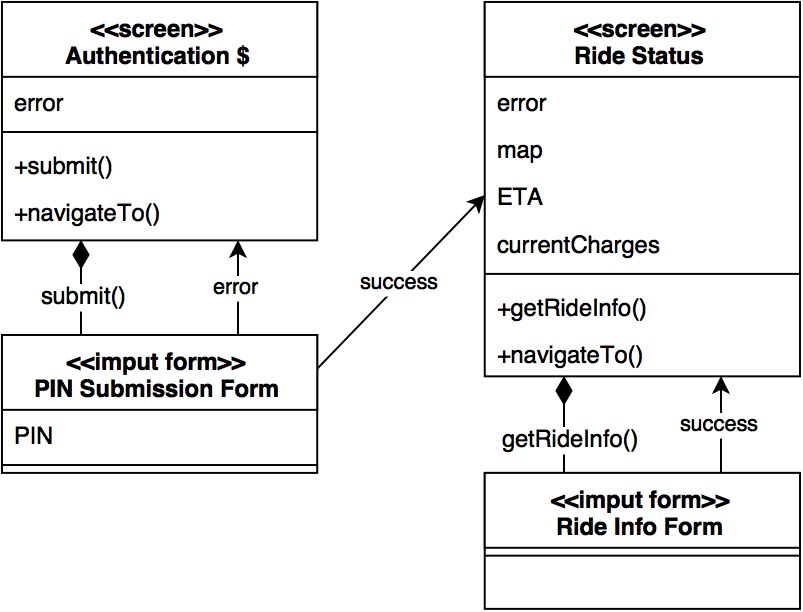
\includegraphics[width=0.4\textwidth]{/DD/OB_ux_schema}\\
		  \vspace{0.4cm}
		  \caption{UX scheme for the on-board application} 
		  \label{fig:OB_ux_scheme} 
		\end{figure}

		After authenticating using his Personal Identification Number, a screen is displayed to the user containing the ride-status informations (which are continuously refreshed through 'getRideInfo').


	\subsection{Mobile/Web application}
		\begin{figure}[!ht]
		  \centering
		  \vspace{0.2cm}
		  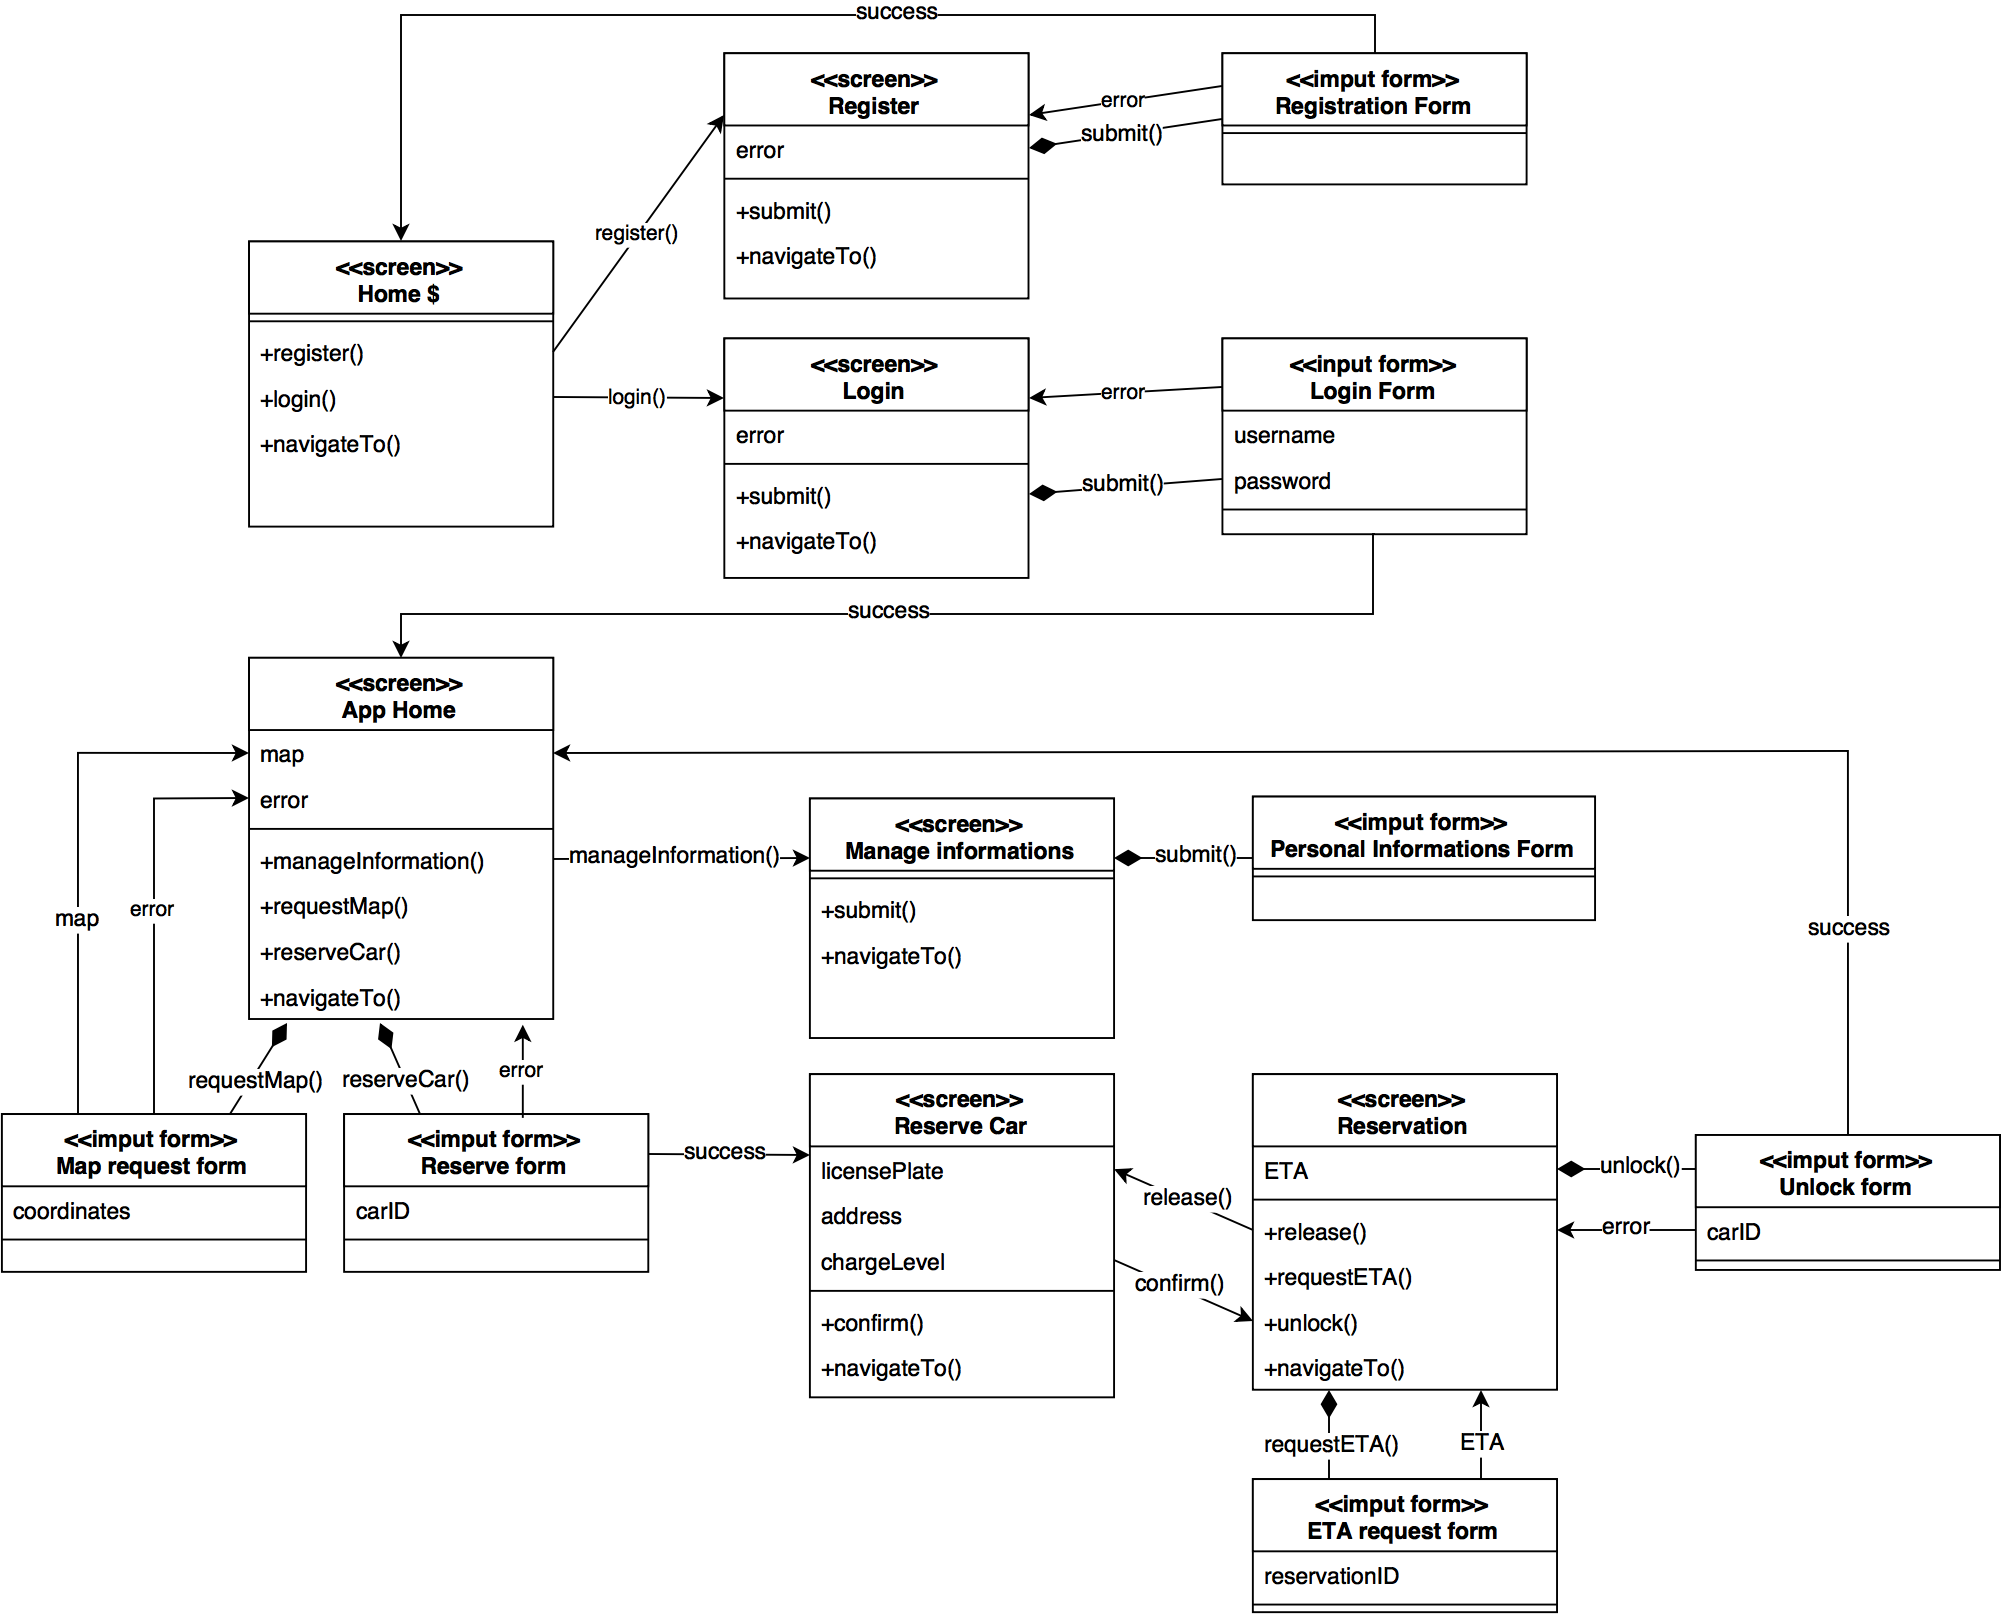
\includegraphics[width=1.0\textwidth]{/DD/ux_schema}\\
		  \vspace{0.4cm}
		  \caption{UX scheme for the mobile and web applications} 
		  \label{fig:ux_scheme} 
		\end{figure}

		After the registration/login the app home page is presented: this screen comprehend a map where all the available cars, safe area and charging stations (which are contained in the 'map' object and continuously refreshed through 'requestMap') are displayed. The user can either navigate to the 'Manage Informations' screen (where he can consult and edit his personal informations) or reserve a car after selecting it on the map. The car is tagged as 'RESERVED' after the user's confirmation and then a 'Reservation' screen is displayed: a timer shows up and the user can Release the reservation or proceed with the Unlock.
		\\When the ride ends the payment is automatically authorized and processed without any user action.


    \chapter{Requirements Traceability}
    	\begin{center}
	\vspace{0.6cm}
	\begin{tabular}{|l|l|l|}
		\hline
		RASD Goals & RASD Functions & DD Component \\\hline
		\hline
		G1, G2, G3 & Registration, Login, Account Management & UserController \\\hline
	\end{tabular}
\end{center}


	% Insert a break for the table of contents
    %\addtocontents{toc}{\protect\newpage}

    % Set page numbering to arabic and restart it before appendix
    \clearpage
	\pagenumbering{Roman}
	\setcounter{page}{1}

	\blankpage

    \appendix
    \newpage
    \chapter{Appendix A: Used Tools}
	    \section{\LaTeX}
Used to format and redact this document
\section{\textit git}
Used as version control system in order to lead development
\section{\textit draw.io}
Used to draw mockups and diagrams
\section{\textit Alloy analyzer}
Used to analyze and verify our specification

	\newpage
	\chapter{Appendix B: Hours of work}
	    These are the hours of work spent by each group member in order to redact this document:
\begin{itemize}  
\item Ruaro Nicola: \worktimeNicola \ hours
\item Gregori Giacomo: \worktimeGiacomo \ hours
\item Total worktime: \worktimeTotal \ hours
\end{itemize}


	\newpage
	\chapter{Appendix C: Revisions}
	    These sections will be eventually redacted during future post-release updates in order to approach the DD modifiability providing a comfortable and higly effective way to trace changes:
\section{Glossary}
	\begin{itemize}
		\item \textbf{v1.1} MVC and JAX-RS entries have been fixed
		\item \textbf{v1.1} Add Notification Handler in architecture diagram
		\item \textbf{v1.2} Update the ER schema and the relation schema associated with it
		\item \textbf{v1.2} Figure 2.8:"Sequence diagram for the reservation’s expiration" has been fixed
		\item \textbf{v1.2} Figure 2.12:"Sequence diagram for the charges computation and application" has been fixed
	\end{itemize}

	% Glossary entries
\newglossaryentry{charging station}
{
  name={charging station},
  description={an area used to re-charge and store electric cars},
  plural={charging stations}
}

\newglossaryentry{ID}
{
  name={ID},
  description={unique identifier associate to an user},
  plural={IDs}
}

\newglossaryentry{pwd}
{
  name={pwd},
  description={User's password, used for acess to the system},
  plural={IDs}
}

\newglossaryentry{safe area}
{
  name={safe area},
  description={Area where PowerEnJoy cars can be parked},
  plural={safe areas}
}

\newglossaryentry{reservation}
{
  name={reservation},
  description={An arrangment to secure availability of a car. An User have to reserve a car before to use it},
  plural={reservations}
}


\newglossaryentry{registration}
{
	name={registration},
	description={The act of a Guest of registering in PowerEnJoy. A Guest, after this operation, became an User},
	plural={registrations}
}
\newglossaryentry{payment}
{
	name={payment},
	description={The act of an User who is paying the system for its service. The payment information are given by the User during her \gls{registration}, they can be changed}
	plural={payments}
}
\newglossaryentry{locking}
{
	name={locking},
	description={The action of the system that automatically lock a car},
}
\newglossaryentry{un-locking}
{
	name={un-locking},
	description{The action of the system that automatically un-lock a car}
}

\newglossaryentry{car-sharing}
{
	name={car-sharing},
	description={Is a model of car rental where people rent cars for short periods of time}
}

\newglossaryentry{bill}
{
	name={payment},
	description={An amount of money that an user gives to the system for the service supplied or for fees}
	plural={bills}
}

\newglossaryentry{notify}
{
	name={notify},
	description={The act of sending a notification}
}
\newglossaryentry{notification}
{
	name={notification},
	description={A message sent by the system to an user for inform him about something important, like a reservation or a payment. It can be an e-mail, banners or messagges}
	plural={notifications}
}

\newglossaryentry{available}
{
	name={available},
	description={A car is tag available when no user is using it or has reserved it. It can also be defined free}
}
\newglossaryentry{FREE}
{
	name={free},
	description={A car is tag free when no user is using it or has reserved it. It can also be defined available}
}
\newglossaryentry{reserved}
{
	name={notification},
	description={A car is tag reserved when an user did a reservation on that car}
}

\newglossaryentry{IN USE}
{
	name={in use},
	description={A car is tag in-use when an user is using it, from the unlock to the lock of the car}
}
\newglossaryentry{OUT OF SERVICE}
{
	name={out of service},
	description={A car is tag out of service when it is parked outside a safe area or when it is left with low battery}
}
\newglossaryentry{payment information}
{
	name={payment information},
	description={Information about the way each user is going to pay the system }
}
\begin{comment}
\newglossaryentry{battery}
{
  name={battery},
  description={},
  plural={batteries}
}
\end{comment}



% Acronyms entries
\newacronym{gps}{GPS}{Global Positioning System}

	\glsaddall
	\printglossaries

	\newpage
	\begin{thebibliography}{10}
		\bibitem{sw-eng2-rules}
	Luca Mottola and Elisabetta Di Nitto, \emph{Software Engineering 2: Project goal, schedule and rules}, 2016
\bibitem{sw-eng2-ci}
	Luca Mottola and Elisabetta Di Nitto, \emph{Assignment 3: Code Inspection}, 2016
\bibitem{ofbiz}
	Apache OFBiz®, \emph{org.apache.ofbiz.service.mail.JavaMailContainer.java}, 2016
	
	\end{thebibliography}

\end{document}
